\documentclass{beamer}
\usepackage[utf8]{inputenc}
\graphicspath{ {./10-presentation-furbeck} }

\title{So who exactly is Becca Furbeck?}
\author{A presentation by Becca Furbeck}
\institute{University of Nebraska-Lincoln}
\date{2020}

\begin{document}

\frame{\titlepage}
\begin{frame}
\frametitle{Who am I?}
This is where I enter text for the frame.
\end{frame}

\begin{frame}
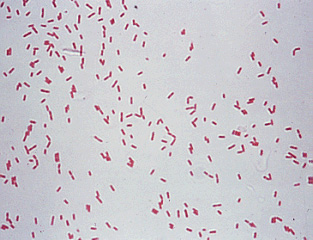
\includegraphics{Pseudomonas}

My favorite animal is \emph{Pseudomonas}. Okay, \emph{Pseudomonas}, is not an animal, but it is the bacteria I study, so I like it more than pretty much every animal...except maybe the ones I obtain it from...
\end{frame}

\end{document}
